\begin{figure*}[t]
\centering
\begin{minipage}[t]{0.315\textwidth}\centering
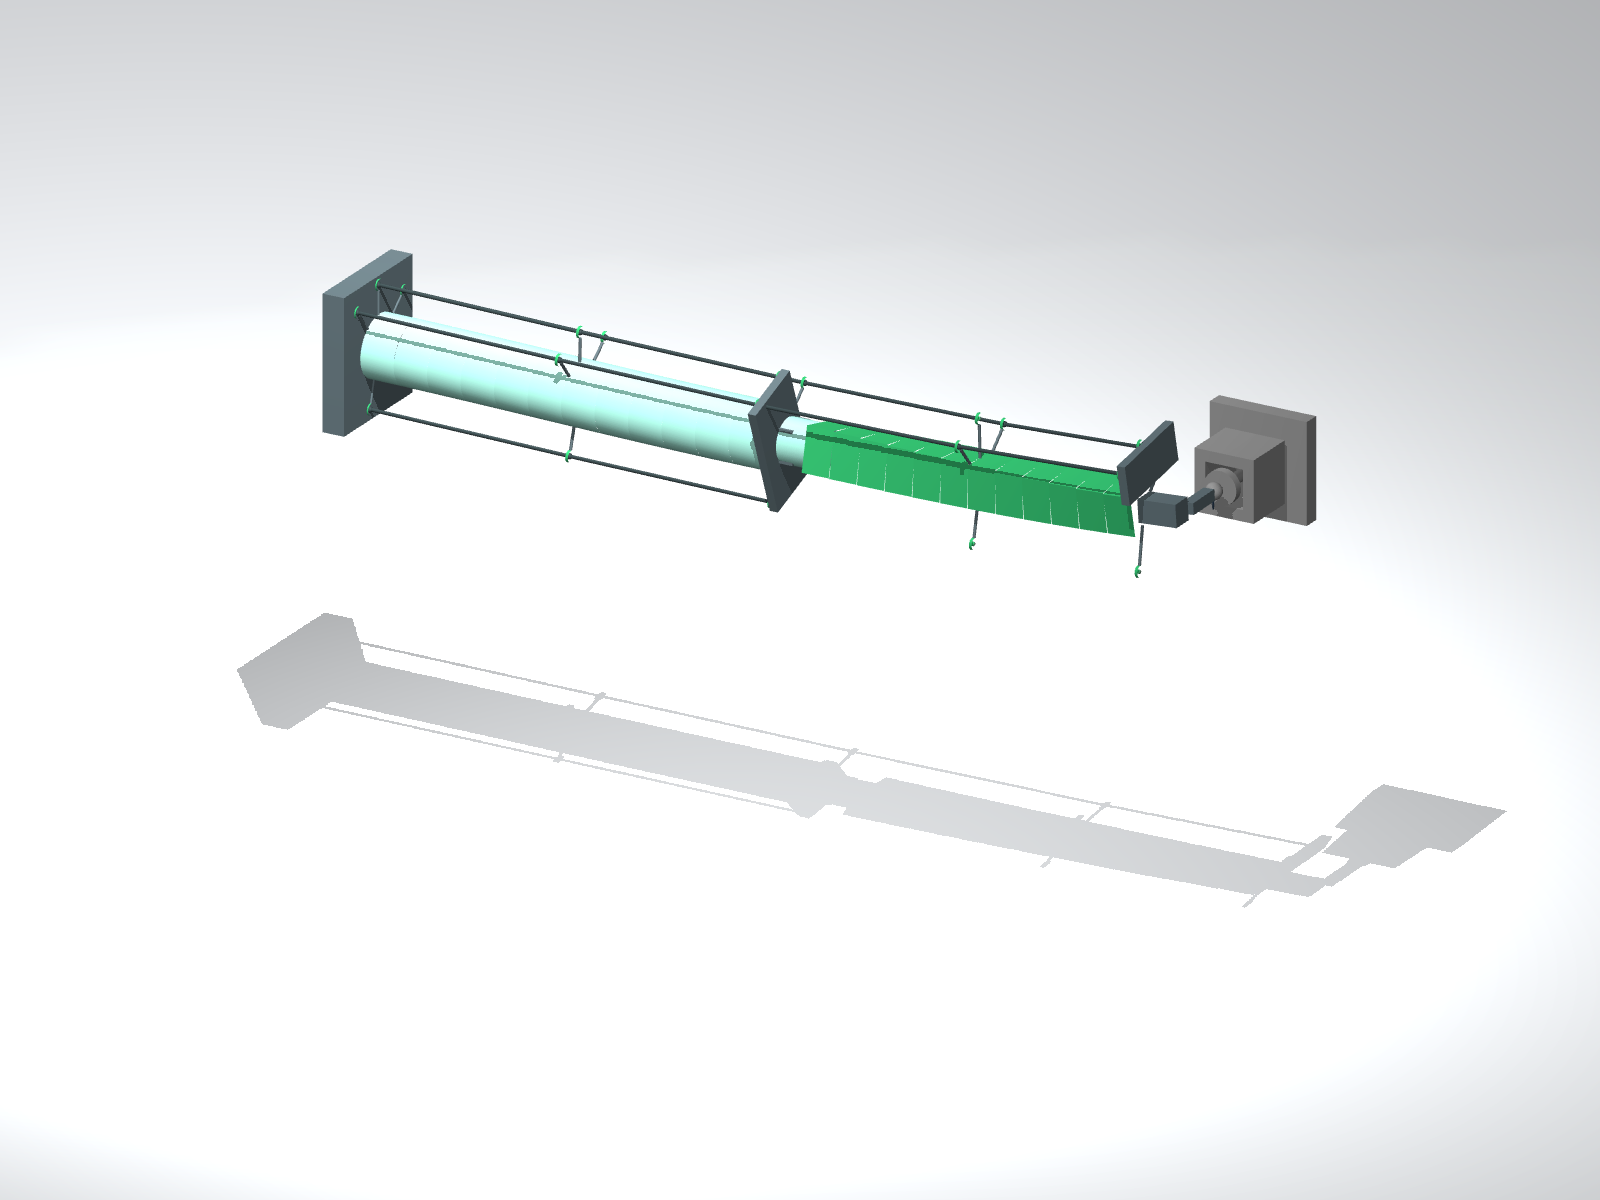
\includegraphics[width=\linewidth]{figures/native/t09_approach.png}
\par\footnotesize (a) Approach
\end{minipage}\hfill
\begin{minipage}[t]{0.315\textwidth}\centering
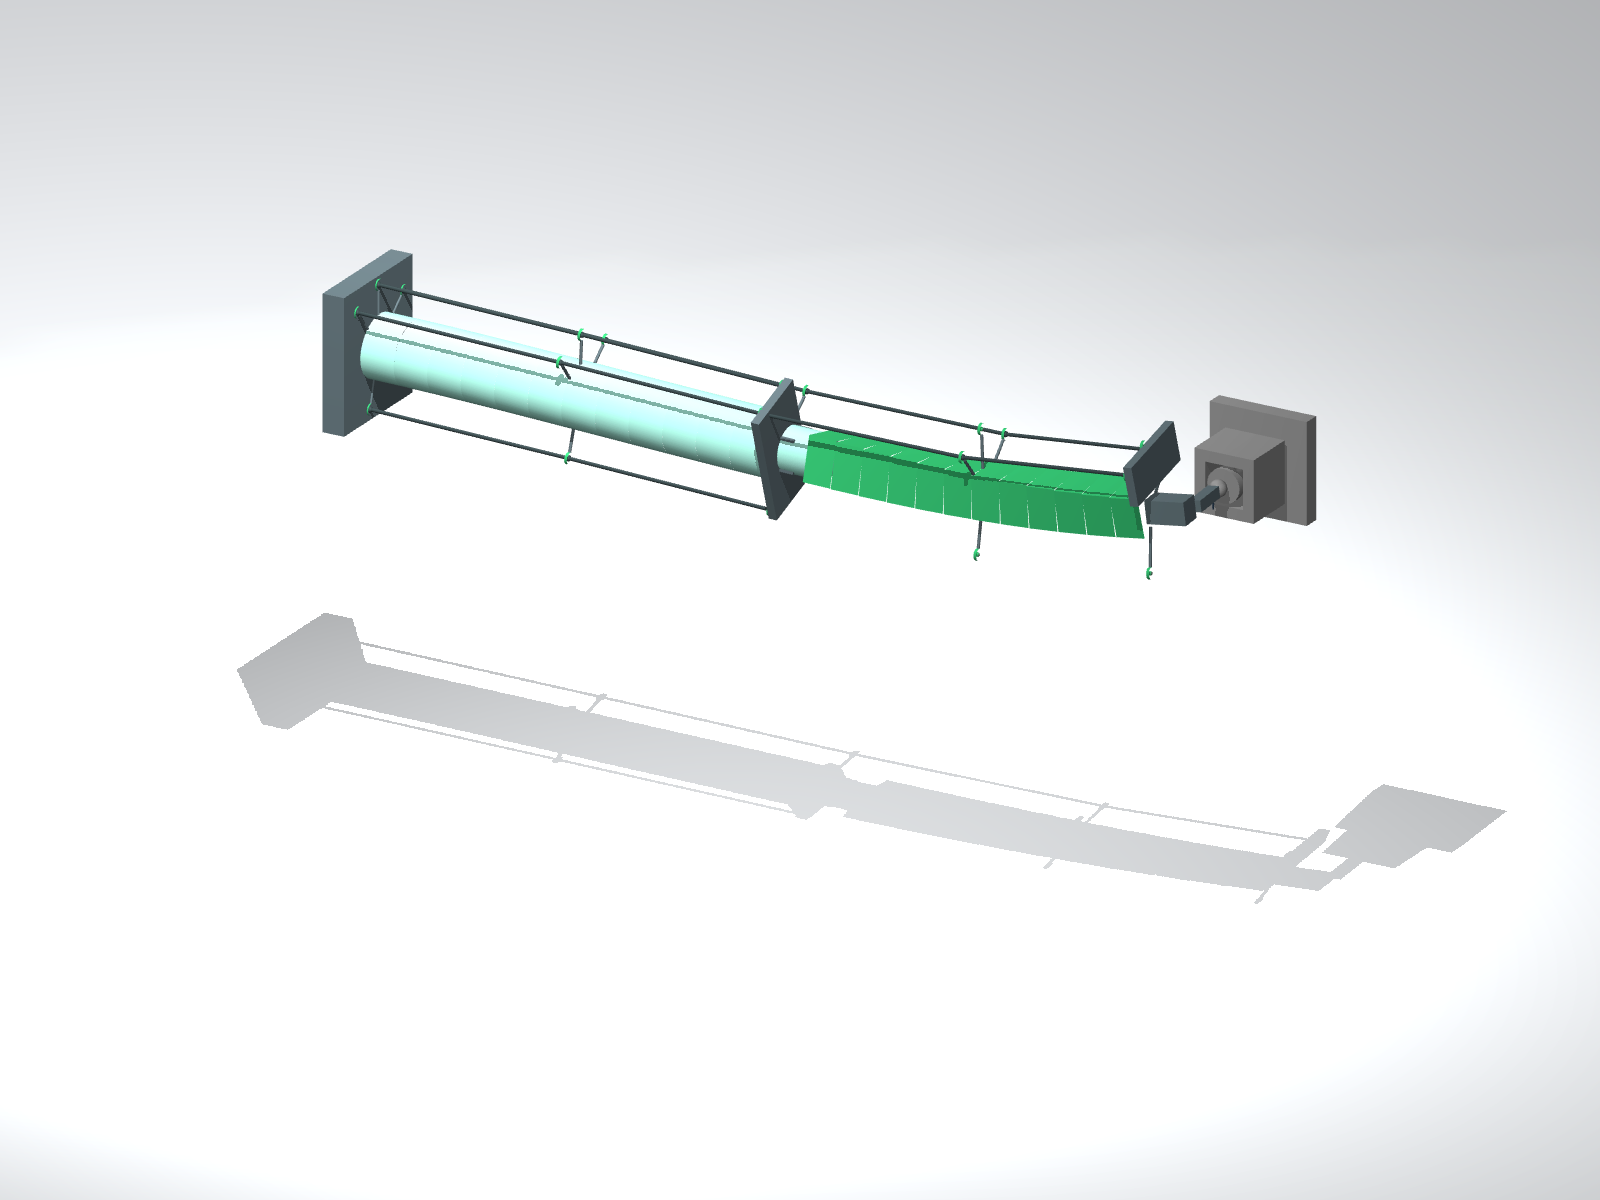
\includegraphics[width=\linewidth]{figures/native/t09_maximum_depth.png}
\par\footnotesize (b) Maximum button travel
\end{minipage}\hfill
\begin{minipage}[t]{0.315\textwidth}\centering
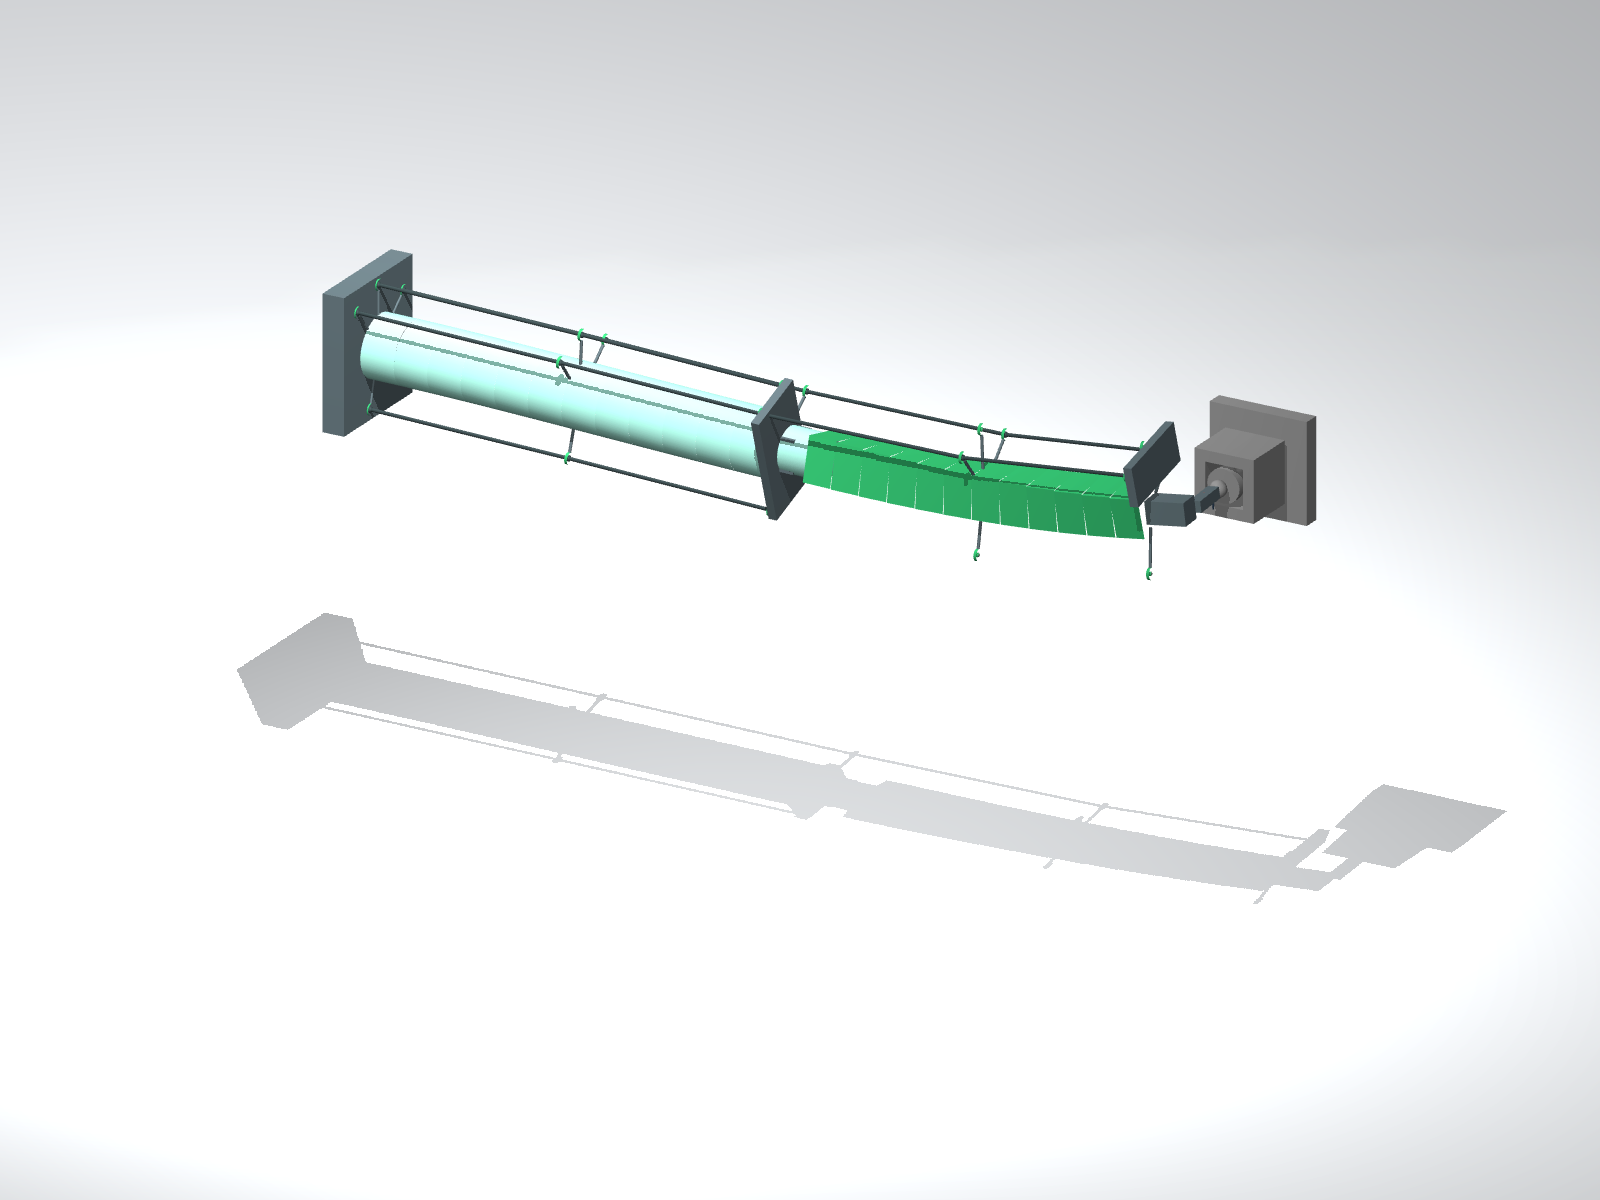
\includegraphics[width=\linewidth]{figures/native/t09_hold.png}
\par\footnotesize (c) Joint depth/force hold
\end{minipage}
\par\vspace{4pt}
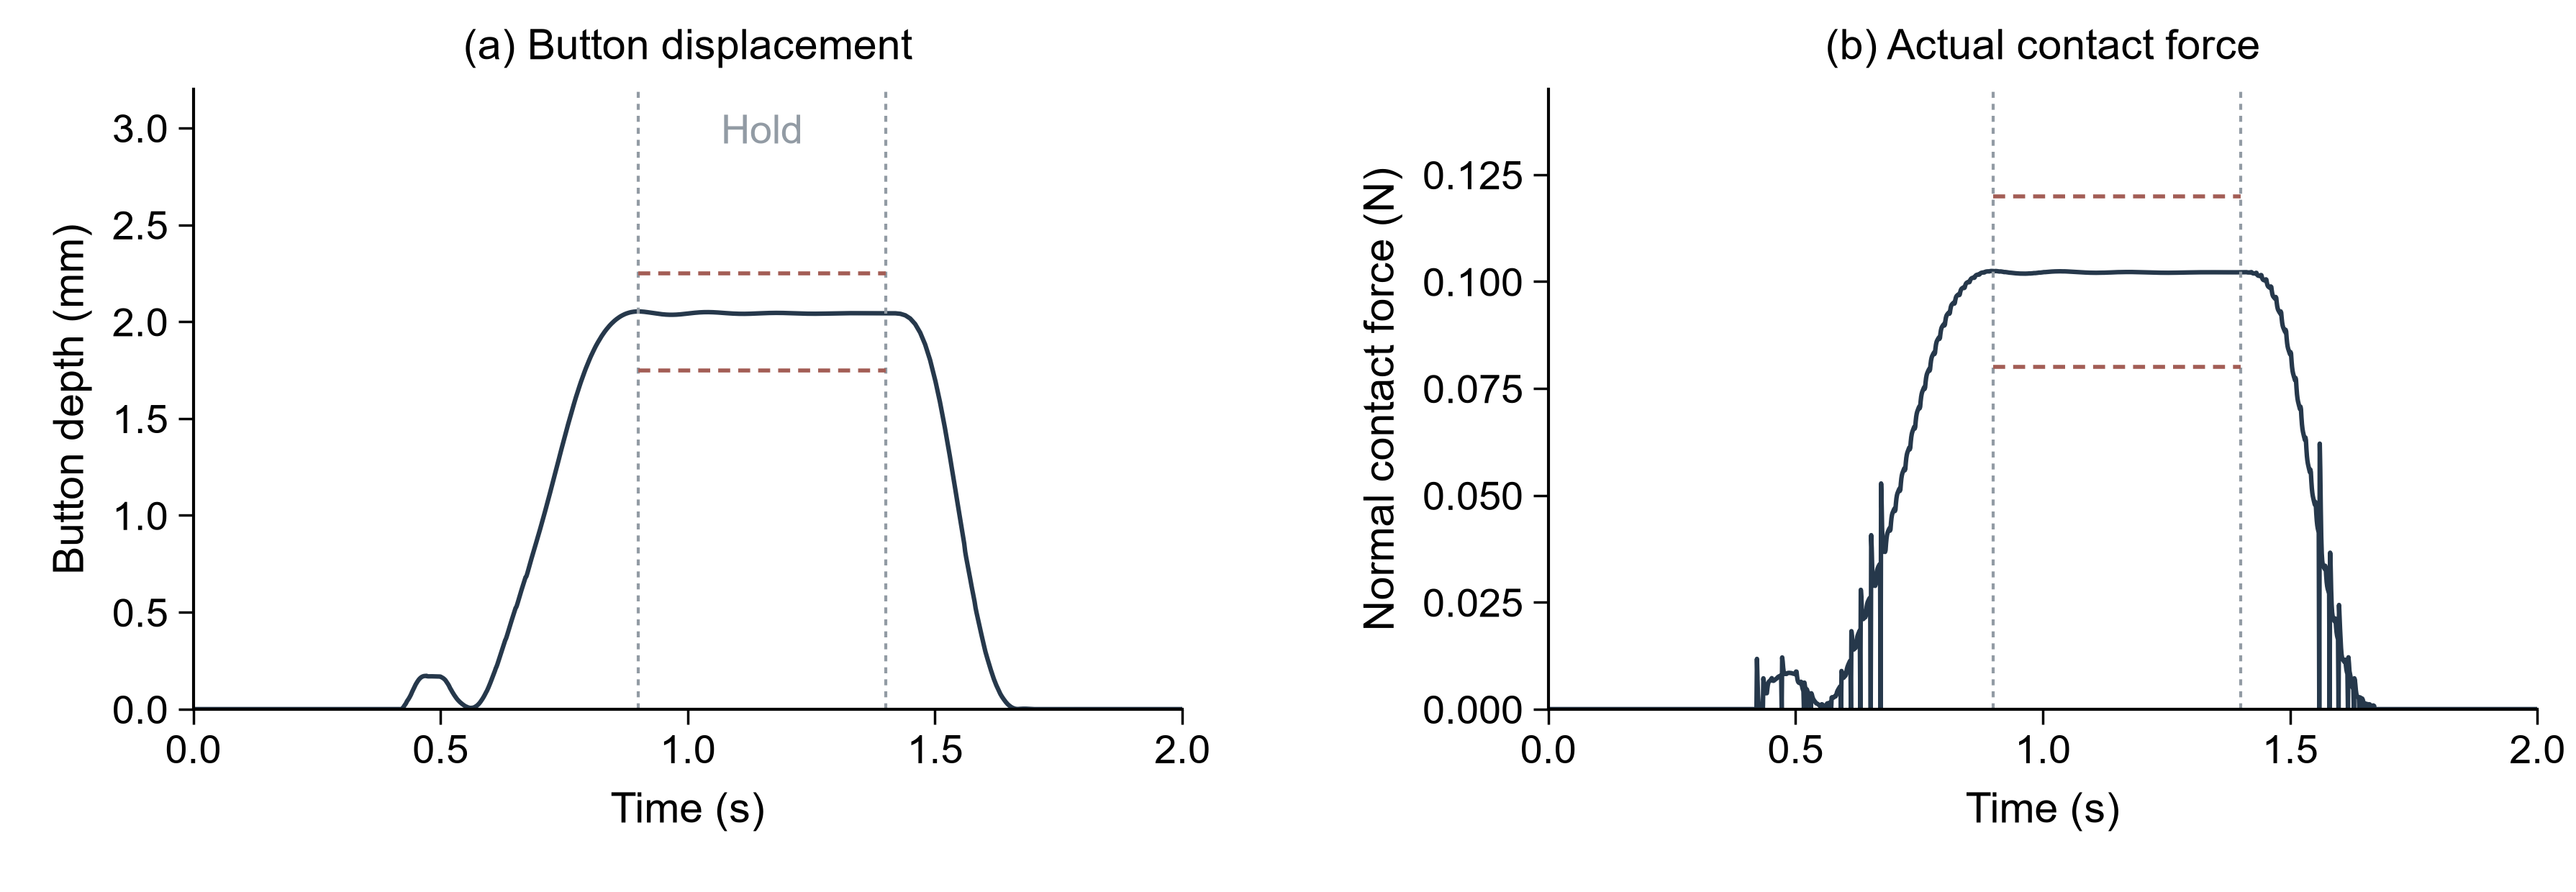
\includegraphics[width=0.88\textwidth]{figures/native/t09_contact_curves.png}
\caption{Native MuJoCo states and measured contact response for T09. The recorded sequence shows approach, maximum button travel, and the joint depth/force hold. The accepted execution maintains the required 0.5-s hold, with maximum depth and contact-force errors of 0.0528~mm and 0.00247~N, respectively.}
\label{fig:physical-execution}
\end{figure*}